\section{Das Experiment}
\subsection{Das Spektrometer}
Ein NMR-Spektrometer besteht aus zwei miteinander verbundenen Teilen, dem Sender- und Empf\"{a}ngerkreis.
Der Senderkreis ist zur Erzeugung der HF-Pulse verantwortlich und der Empf\"{a}ngerkreis detektiert das Kernspininduktionssignals.

Der Aufbau des Senderkreises ist in Abbildung (\ref{senderkreis.}) schematisch dargestellt.
Mit dem HF-Generator (1) wird ein Signal mit Lamorfrequenz generiert, welches \"{u}ber zwei schalter (3) geschickt wird.
Diese Schalter werden zeitlich vom Pulsgenerator (2) so gesteuert, dass die HF-Pulse mit der richtigen L\"{a}nge aus dem kontinuierlichen Signal erzuegt werden.
Die HF-Pulse werden \"{u}ber (4) zim Leistungsverst\"{a}rker gef\"{u}hrt.
Um zu gew\"{a}hrleisten, dass nur die eintreffenden Pulse um den Faktor $10^6$ verst\"{a}rkt werden, besitzt der Leistungsverst\"{a}rker einen weiteren Eingang, den Gating-Eingang.
Der Pulsgenerator kann \"{u}ber diesen zweiten Eingang den Verst\"{a}rker gezielt ein- und ausschalten.
\"{U}ber ein Kabel (6) werden die verst\"{a}rkten HF-Pulse dann zur Probe geleitet.
\setcounter{figure}{10}
\begin{SCfigure}[1][!h]
	\centering
	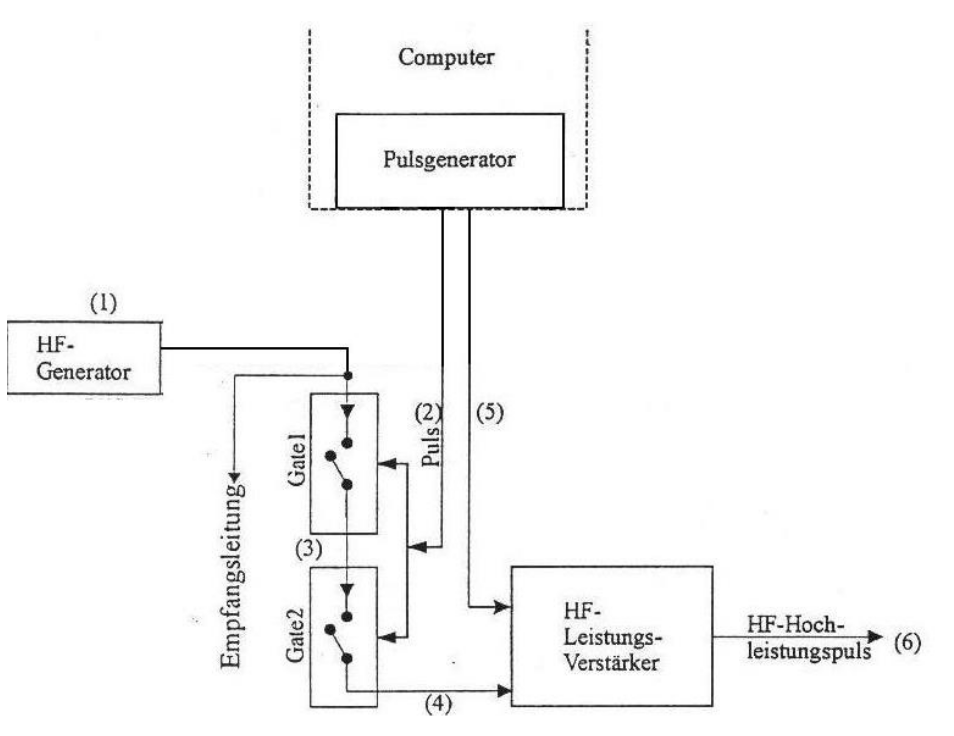
\includegraphics[width=0.6\textwidth]{Plots/spektrometer.png}
	\caption{Aufbau des Senderkreises zur Erzeugung der HF-Pulse. (1) erzeugt ein HF-Signal. \"{U}ber (2) und (5) kann der Pulsgenerator die Schalter und den Vorverst\"{a}rker zeitlich ansteuern. Mittels der Schalter (3) wird ein HF-Puls generiert, welches zum Vorverst\"{a}rker (4) gef\"{u}hrt wird. Und \"{u}ber (6) kann der HF-Puls  zur Probe gef\"{u}hrt werden (siehe Versuchsanleitung \cite{Anleitung}[S.28]).}
	\label{senderkreis.}
\end{SCfigure}

Damit HF-Pulsen in der Probenspulen ein maximales $B_1$-Magnetfeld erzeugen, muss m\"{o}glichst viel Leistung in den Probenstab gebracht werden.
Hierf\"{u}r ist zum einen die Abstimmung des Probenkopfs wichtig und zum anderen wird eine Kombination aus einem $\lambda / 4$-Kabel und zwei Diodenp\"{a}archen ben\"{o}tigt, siehe Abbildung (\ref{lambda4.}).
W\"{a}hrend der Zeit eines HF-Pulses liegt an dem Diodenp\"{a}archen (A) eine so hohe Spannung an, dass diesen den ankommenden HF-Puls durchgelassen.
Das $\lambda /4$-Kabel bewirkt f\"{u}r diese Zeit durch eine Impedanztransformation einen unendlich hohen Wellenwiderstand, sodass die Welle des HF-Pulses den Weg in den Probenstab nehmen muss.
Anders als bei dem kleinen Kerninduktionssignal, hier sperrt das Diodenpaar (A).
Um zu 
\begin{wrapfigure}[10]{r}{0.5\textwidth}
	\centering
	\framebox[0.45\textwidth]{
	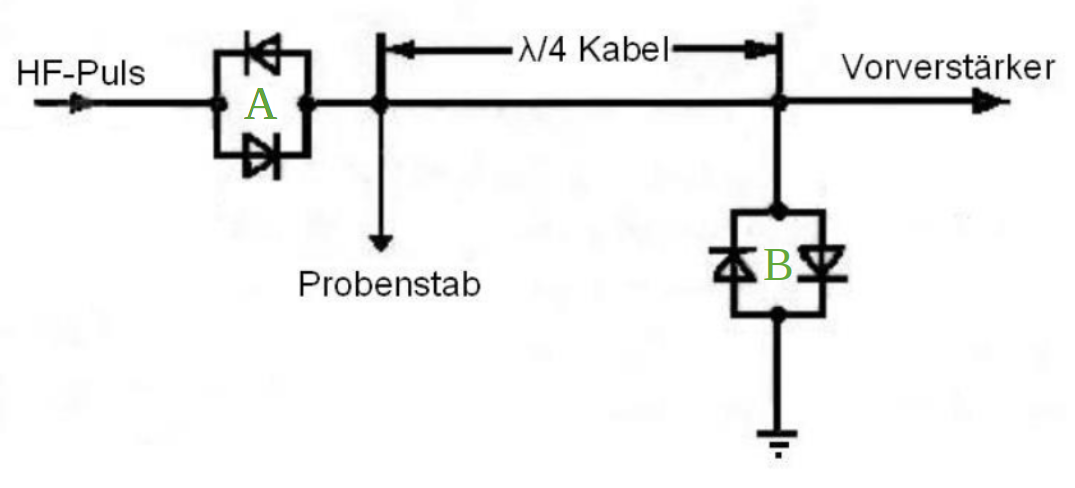
\includegraphics[width=0.4\textwidth]{Plots/diodengruen.png} }
	\caption{Schaltbild des $\lambda / 4$-Kabels (siehe Versuchsanleitung \cite{Anleitung}[S.28]).}
	\label{lambda4.}
\end{wrapfigure}
gew\"{a}hrleisten, dass das Kerninduk{\-}tions{\-}sig{\-}nal vollst\"{a}ndig zum Vorverst\"{a}rker gelangt, ist ein zweites Diodenpaar (B) in der Sendeleitung eingebaut.
Auch dieses l\"{a}sst nur hochfrequente Pulse durch und sperrt f\"{u}r das kleinen Kerninduktionssignal.
Anders ausgedr\"{u}ckt verhindert das Dioden{\-}paar (B), dass starke Pulse in den Vorverst\"{a}rker gelangen k\"{o}nnen und ist f\"{u}r die Impe{\-}danz{\-}trans{\-}formation wichtig.
Zus\"{a}tzlich wird das Restrauschen des Leistungsverst\"{a}rker von dem Diodenpaar (A) nicht durchgelassen.
Eine weitere sehr wichtige Funktion des $\lambda / 4$-Kabels ist das Umschalten von Sende- zu Empfangssignal und andersherum.

\paragraph{Probenkopf}
\begin{wrapfigure}[13]{r}{0.35\textwidth}
	\centering
	\framebox[0.3\textwidth]{
	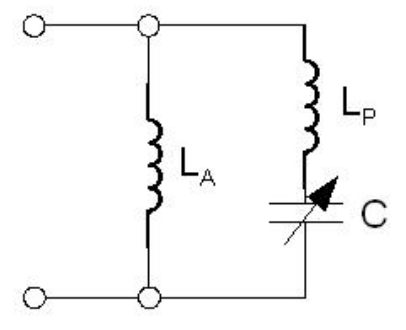
\includegraphics[width=0.25\textwidth]{Plots/schwingkreis.png} }
	\caption{Schaltbild des Reihenresonanzkreis im Probenkopf (siehe Versuchsanleitung \cite{Anleitung}[S.30]).}
	\label{probenkopf.}
\end{wrapfigure}
Der Aufbau des Probenkopfes bestehlt aus einem Reihenresonanzkreis.
Die Resonanzfrequenz entspricht hierbei der Lamorfrequenz und die Impedanz ist auf $50 \Omega$ justiert.
In Abbildung (\ref{probenkopf.}) ist der Reihenresonanzkreis schematisch dargestellt.
Die Probenspule $L_P$ ist Teil des Schwingkreises.
Auf Grund dessen muss die Resoanzfrequenz vor jeder Messung und auch nach jeder Temperatur\"{a}nderung erneut angepasst werden.
Die Anpassung erfolgt \"{u}ber ein Netzwerkanalysator, der das Stehwellenverhältnis (VSWR) misst.
Diese l\"{a}sst sich auch wie folgt aus den Spannungsamplituden aus der tranmitterten ($U_T$) und der reflektierten ($U_R$) Welle berechnen:
\begin{align*}
	\text{VSWR} = \frac{U_T + U_R}{U_T - U_R} .
\end{align*}
Eine optimale Impedanzanpassung wird bei VSWR = 1 erreicht.

\paragraph{Detektions}
Das zu detektierende Kerninduktionssignal $\omega_{RF}$ besitzt eine Frequenz im MHz-Bereich.
F\"{u}r die direkte Detektion so hoher Frequenzen werden schnellen Analog-Digital Wandler ben\"{o}tigt.
Diese Analog-Digital Wandler bestitzen jedoch nur ein schlechtes Aufl\"{o}ungsverm\"{o}gen.
Zur L\"{o}sung des Probles wird das Kerninduktionssignal mit dem Signal der Hochfrequenzquelle gemischt und in zwei Komponenten zerlegt.
Die erste Komponente ist die Summe der beiden Kreisfrequenzen, $\omega_1 = \omega_L + \omega_{RF}$, und die zweite Komponente ist die Differenzfrequenz, $\omega_2 = \omega_L - \omega_{RF}$.
Mittels eines Tiefpassfilters wird die niederfrequente Komponente $\omega_2$ herausgefiltert.
Im n\"{a}chsten Schritt l\"{a}sst sich $\omega_2$ nun exakt digitalisieren.
Da lediglich die Differenfrequenz analysiert wird, kann dadurch experimentell nicht geschlussfolgert werden welche der beiden Frequenzen gr\"{o}{\ss}er beziehungsweise kleiner ist.
Um diese H\"{u}rde zu \"{u}berwinden wir einen Quadraturdetektion durchgef\"{u}hrt.
Hierbei wird das Kerninduktionssignal zus\"{a}tzlich noch mit einem um $90^{\circ}$ phasenverschobenen Signal gemischt.
In der NMR werden die Komponenten, die sich daruch ergeben, mit Real- und Imagin\"{a}rteil gekennzeichnet.
%\begin{figure}[hbtp]
%	\centering
%	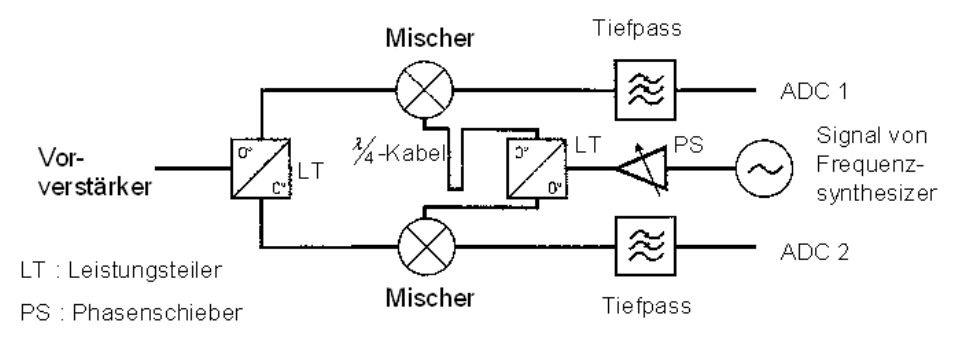
\includegraphics[width=0.5\textwidth]{Plots/mischer.png}
%	\caption{.}
%	\label{.}
%\end{figure}


\subsection{Durchf\"{u}hrung}
Bevor mit der ersten Messung gestartet werden kann, wird dir Probe in den Probenkopf eingesetzt.
Dieser wird dann in das NMR-Spekrometer eingebaut.
Um im ersten Schritt den Probenkopf abzustimmen, wird dieser mit einem Netzwerkanalysator verbunden und das Stehwellenverh\"{a}ltnis (VSWR) zu bestimmen.
%oder war das ein Oszilloskop?
F\"{u}r die weiteren Messungen wird der Probenkopf mit dem $\lambda / 4$-Kabel und den Steuerger\"{a}ten verbunden.

Alle Messungen werden \"{u}ber ein Python-Skript angesteuert.
Experimente k\"{o}nnen ausgew\"{a}hlt und Variablen, so wie beispielsweise die $t_p$-Zeit, ver\"{a}ndert werden.
So werden die Pulsl\"{a}nge eines $180^{\circ}$-Pulses, die $T_1$- und die $T_2$-Relaxationszeit bestimmt.

Im zweiten Teil des Versuches wird ein stimuliertes Echo f\"{u}r verschiedene Temperaturen gemessen.
Zun\"{a}chst m\"{u}ssen hierf\"{u}r alle Parameter bestmmt und eingestellt werden.
%310-345 in 3K schritten
